\chapter{Precision Medicine in Ischemic Heart Disease}
\label{chap:precision-medicine}

Ischemic heart disease is a term covering a variety of conditions, 
all caused by myocardial ischemia---%
an imbalance between the coronary blood supply and the 
oxygen requirements of the myocardium.
In the overwhelming majority of cases, 
this imbalance can be attributed to obstructive atherosclerotic disease 
that limits coronary blood flow
\sidecite[-2em]{kumarRobbins2014}.
In these cases, ischemic heart disease is therefore synonymous 
with coronary artery disease.

The central etiological entity in ischemic heart disease
is therefore the atherosclerotic plaque
\sidecite[-2em]{kumarRobbins2014}
An atherosclerotic plaque consists of blood cells, lipids, calcium 
and connective tissue that are gradually deposited in the arterial wall 
over a number of years.
\sidecite[-4em]{libbyPathophysiology2005}
The plaque can grow large enough to severely narrow the arterial lumen,
or it can become unstable and as a consequence rupture or erode,
leading to thrombosis.%
\sidecite[-3em]{fusterPathogenesis1992}
Both of these scenarios can severely affect 
the perfusion of tissues and organs, 
and when coronary arteries are affected,
it leads to ischemic heart disease.

% figure: atherosclerosis→
\begin{figurefw}
    \centering
    \vspace{-5em}
	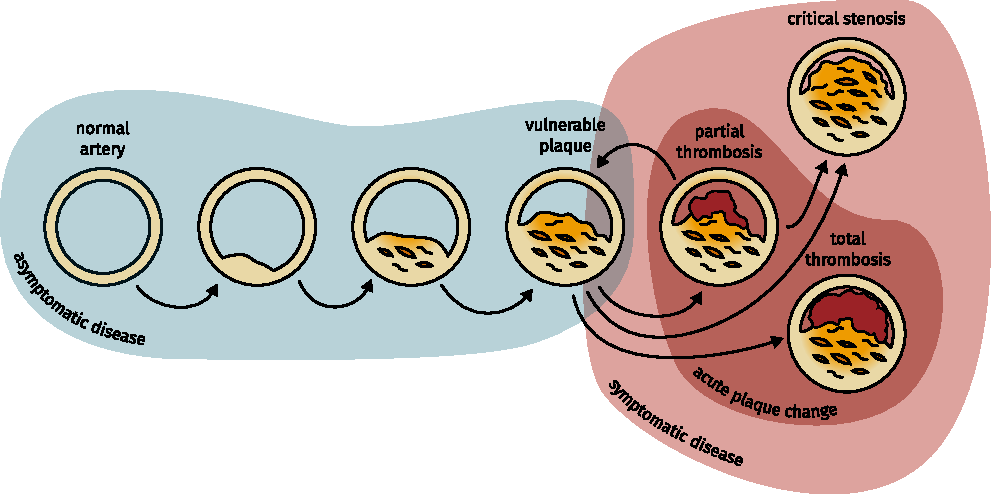
\includegraphics[width=\linewidth]{graphics/atherosclerosis}
    \caption[The atherosclerotic process]{%
        The atherosclerotic process. 
        From a otherwise normal artery, 
        disruption of endothelial integrity and function, 
        through a combination of genetics and risk factors,
        leads to endothelial injury and low-grade inflammation. 
        Over time, this results in plaque formation through 
        accumulation of lipids, lipoproteins, calcium, and connective tissue.
        Eventually, the plaque may become \enquote{vulnerable}, 
        making it susceptible to sudden rupture or erosion. 
        Such an event can trigger thrombosis and acute changes in the plaque, 
        which, depending on their severity, may either immediately obstruct 
        the arterial lumen%
        ---leading to myocardial infarction or sudden cardiac death---%
        or contribute to further calcification through remodeling. 
        When the progressive narrowing of the arteries reaches a point where 
        it causes symptoms, the stenosis is considered critical, and the 
        myocardium experiences inadequate perfusion, manifesting as 
        ischemic heart disease.
    }
    \vspace{-5.1em}
    \label{fig:atherosclerosis}
\end{figurefw}
\vspace{9em}% ←

\section{Disease Manifestation}

The pathological process underlying ischemic heart disease 
is inherently chronic with atherosclerotic lesions 
gradually developing over time, 
but in the event of plaque rupture it can abruptly transition
and manifest as an acute condition.
The clinical presentation of ischemic heart disease  
is consequentially diverse and includes both acute 
~\autocite{byrne20232023}
and chronic coronary syndromes.
~\autocite{knuuti20192020}

Acute coronary syndromes includes 
\ac{UA}, \ac{STEMI}, and \ac{NSTEMI},
that collectively represents a spectrum of acute onset or progression of 
myocardial ischemia.
If the ischemia is sufficient to cause myocardial necrosis, 
it is per definition called \ac{MI}~\autocite{thygesenFourth2019}.
\ac{STEMI} and \ac{NSTEMI} are both forms of \ac{MI} that are distinguised
by a characteristic presence or absence of ST-segment elevation on a \ac{ECG}.
All of the acute coronary syndromes are typically associated 
with acute plaque change and atherothrombosis, 
and are medical emergencies that require immediate 
intervention to limit or prevent myocardial damage.
~\autocite{kumarRobbins2014}

% figure: ecg→
\begin{marginfigure}%
    \vspace{1em}
    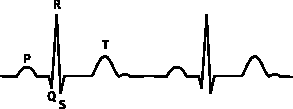
\includegraphics{graphics/electrocardiogram}
    \caption[An example electrocardiogram]{%
        Schematic of a normal sinus rhythm as seen from an ECG. 
        In \ac{STEMI}, the ST-segment is found elevated.
    }
    \vspace{1em}
    \label{fig:ecg}
\end{marginfigure}% ←

Chronic coronary syndromes are more stable manifestations of the disease,
and include stable angina and chronic ischemic heart disease.
Stable angina, or \textit{angina pectoris}, is characterised by episodes of
crushing chest pain caused by myocardial ischemia, initially typically during
exercise.
By definition, the level of ischemia is not severe enough to lead to
tissue necrosis. 
~\autocite{knuuti20192020}
Unlike \ac{UA}, the symptoms of stable angina are often more predictable,
reliably triggered by a specific level of physical exertion, 
and typically absent when the individual is at rest. 
Chronic ischemic heart disease can either be a long-term progression of stable
ischemic heart disease or a late-stage stabilization following a \ac{MI} that
has undergone revascularization. 
~\autocite{knuuti20192020}
This condition represents the cumulative
effects of prolonged myocardial ischemia and accrued myocardial damage,
ultimately leading to progressive congestive heart failure.
~\autocite{kumarRobbins2014}

\section{Diagnosis and Treatment}

Since the 1950s, a series of groundbreaking scientific advances have improved 
our understanding and management of cardiovascular disease, leading to a 
drastic decline of mortality in ischemic heart disease.
~\autocite{nabelTale2012}
These advances span from from diagnostic imaging techniques to pharmacological
interventions and surgical procedures, each contributing to a more nuanced
understanding of the disease and more effective treatment options.
~\autocite{nabelTale2012}
To translate this constantly evolving body of knowledge into actionable medical
practice, the European Society of Cardiology (ESC) annually releases
comprehensive clinical practice guidelines that cover a wide array of
cardiovascular conditions.

In line with ESC guidelines, 
invasive management is the recommended approach
for immediate treatment of acute coronary syndromes.
This includes primary \ac{PCI}%
% sidenote: pci{{{
\sidenote[][-3em]{%
    \ac{PCI} is a minimally invasive procedure used for treatment of
    atherosclerosis. It involves the use of a small balloon catheter 
    to widen flow-limiting stenoses and restore cardiac perfusion.
} % }}}
for \ac{STEMI} and emergency angiography, 
potentially with concurrent \ac{PCI},
for patients with very high-risk \ac{NSTEMI} and \ac{UA}.
For those with a more stable presentation, but still at high-risk, 
angiography within the first 24 hours is indicated to
assess the need for revascularization. 
~\autocite{byrne20232023}
Based on factors such as the coronary anatomy, 
number and grade of stenotic vessels, 
and the estimated risk of surgical complications
\ac{CABG} is sometimes preferred over \ac{PCI}.
~\autocite{neumann20182019}
The primary objective of these interventions 
is providing timely revascularization where needed,
to restore coronary perfusion and limit myocardial damage.

Contrastingly, for chronic coronary syndromes,
invasive coronary angiography is typically not 
the first-line diagnostic test.
~\autocite{knuuti20192020}
However, for patients with a high clinical likelihood of ischemic heart
disease, who present with easily induceable or refractory angina pectoris 
and a high event risk, coronary angiography is recommended for assessment of
revascularization options.  
~\autocite{knuuti20192020}

Concurrent with invasive treatment, 
the guideline gives a class I recommendation for initiation 
of antithrombotic therapy in patients with \ac{IHD}. 
~\autocite{byrne20232023}
While the specifics of this therapy is beyond the scope of this thesis,
it generally involves a combination of antiplatelet medications, 
aimed at preventing further thrombotic events.
~\autocite{nabelTale2012}

\section{Secondary Prevention}

\marginnote[-2.5em]{%→

\textit{Primary prevention} aims to prevent disease onset, 
often through healthy lifestyle choices. 

\textit{Secondary prevention} focuses on 
managing an existing condition to prevent complications and progession.
}% ←

Once the acute phase of the disease has been stabilized 
through revascularization or other treatments,
the clinical focus shifts to long-term management and secondary prevention.
Patients with established ischemic heart disease are generally of 
high risk of subsequent events, 
particularly if risk factors are not adequately managed.
~\autocite{clarkMetaAnalysis2005}
Guidelines advocate for a multifaceted approach to secondary prevention, 
incorporating lifestyle changes like quitting smoking and starting exercise, 
as well as pharmacological interventions such as lipid-lowering therapies. 
~\autocite{visseren20212021}

The goal of long-term treatment is essentially twofold:
to limit the progression of existing atherosclerotic plaque and 
to prevent and limit thrombus formation if plaques should rupture or erode.
~\autocite{foxMyth2020}
The clinical trajectories of patients with chronic manifestations of 
ischemic heart disease can remain stable for several years,
before unexpectedly deteriorating to 
major adverse cardiovascular events.
~\autocite{foxMyth2020}
Consequently, continuous monitoring and risk factor control 
are recommended to guide secondary prevention therapy.

In this setting,
risk stratification models that combine the clinical characteristics 
and risk factor profiles of the individual patient can be useful.
~\autocite{visseren20212021}
These models could help identify at-risk patients most likely to benefit from 
aggressive therapy. 
However, the real-world application of such models is not without challenges.
There is a need for rigorous validation studies to establish their 
clinical utility, as well as the development of 
protocols for their integration into routine clinical practice.

Additionally, there is a gap in understanding how comorbidities---%
whether cardiovascular or non-cardiovascular---%
affect outcomes and should be factored into treatment planning and prognosis.%
\sidenote[][13em]{\cite{visseren20212021}}
This is where the role of precision medicine becomes particularly salient. 
By leveraging advanced computational techniques and large-scale clinical data,
precision medicine has the potential to fill these gaps.

\section{Perspectives of Precision Medicine}

A 2013 Cochrane review on \citetitle{taylorStatins2013} concluded 
that statins effectively lower all-cause mortality and reduce the incidence
of both fatal and non-fatal cardiovascular events without any serious
adverse effects~\autocite{taylorStatins2013}.
For instance, the relative risk of fatal cardiovascular events 
when using statins as opposed to placebo
was estimated to \num{0.82} with a 
\si{95}{\%} \ac{CI} of \num{0.70} to \num{0.96}.
~\autocite{taylorStatins2013}
This suggests those treated with statins, on average,
are \si{18}{\%} less likely to die from cardiovascular causes. 
However, it is important to emphasize that this \si{18}{\%} 
reduction is an average effect for the \enquote{average individual}.
There might be groups of people for whom the reduction could be 
even higher, while others may see little to no benefit. 
Understanding and making use of such individual variability 
is the central objective of \enquote{precision medicine}.

Precision medicine is broadly speaking an approach to healthcare 
that aims to tailor medical treatment and management to the individual patient.
Instead of employing a \enquote{one-size-fits-all} methodology, 
where treatment and preventive care is being developed to the average patient,
precision medicine uses data-driven approaches to also account for 
the specific factors of the individual.
As such, the underlying idea of precision medicine is not really new;
tissue- and blood typing, for example,  
has been used to guide organ and blood donation for several decades.
However, the prospective of leveraging large clinical databases
and broad array of phenotypic information is adding renewed interest 
in the concept.
~\autocite{collinsNew2015}

% table: pgx-vars →
\begin{table*}[t]
\footnotesize
\centering
\tlfstyle
\begin{tabularx}{\linewidth}{r l p{3cm} X p{3.1cm}} 
\toprule
Gene & Variant & Drug & Description & Reference \\ 
\midrule

ABCG2 
& rs2231142
& rosuvastatin 
& Genotypes GT and TT is associated with increased plasma concentrations of 
rosuvastatin compared to genotype GG. 
&  \href{https://www.pharmgkb.org/clinicalAnnotation/1451666660}{1451666660}
\\

CYP2C9 
& *2 + *3 
& fluvastatin 
& Heterozygous or homozygous mutant allele carriers (*2 or *3) 
have an increased plasma concentration of fluvastatin.
& \href{https://www.pharmgkb.org/clinicalAnnotation/1451666740}{1451666740}
\\

CYP2C9 
& *2 + *3 
& fluvastatin 
& Heterozygous or homozygous mutant allele carriers (*2 or *3) 
have an increased likelihood of adverse events
when treated with fluvastatin compared to CYP2C9 *1/*1. 
&  \href{https://www.pharmgkb.org/clinicalAnnotation/1451678600}{1451678600}
\\

SLC01B1 
& rs4149056 
& rosuvastatin, simvastatin, pravastatin, lovastatin, fluvastatin, atorvastatin
& Genotypes CC and CT is associated with an increased risk of myopathy
when treated with either of the listed statins compared to genotype GG.
& \href{https://www.pharmgkb.org/clinicalAnnotation/1451357200}{1451357200},
\href{https://www.pharmgkb.org/clinicalAnnotation/1451244720}{1451244720},
\href{https://www.pharmgkb.org/clinicalAnnotation/1451244740}{1451244740},
\href{https://www.pharmgkb.org/clinicalAnnotation/1043880818}{1043880818},
\href{https://www.pharmgkb.org/clinicalAnnotation/655384011}{655384011},
\href{https://www.pharmgkb.org/clinicalAnnotation/1451465324}{1451465324}
\\

\bottomrule
\end{tabularx}
\caption[Example statin pharmacogenomic variants]{
	Examples of pharmacogenomics variants related to statin treatment 
	from the PharmGKB database.
	The included variants are all Level 1A clinical annotations, 
	which specify combinations of genetic variants and drugs for which there 
	is targeted prescribing guidance available either in
	current clinical guidelines or in FDA-approved drug labels. 
	Additionally, the Level 1A annotations are required to have a
	minimum of one supporting published article, in addition to the
	variant-specific recommendations.
 }
\label{tab:pgxvars}
\end{table*}% ←

In the context of statin treatment,
this class of medication is generally both
highly effective and very well-tolerated, with limited side effects.
~\autocite{taylorStatins2013}
Some individuals may experience mild side effects such as muscle aches, 
while more severe side effects like myopathy or rhabdomyolysis 
are exceedingly rare.
~\autocite{thompsonStatinAssociated2003}
The underlying mechanism of 
statin-induced skeletal muscle side effects
is not well defined, 
but appears to be connected with the drug's serum concentration.
~\autocite{thompsonStatinAssociated2003}
Pharmacogenomics, a critical component of the pharmacological aspects of 
precision medicine, 
adds another layer to this understanding. 
It explores how genetic factors influence drug response, 
allowing for understanding etiology and more nuanced treatment plans. 
Genome-wide analyses have already identified \acp{SNP} 
that are associated with an increased risk 
of statin-induced side effects (Table \ref{tab:pgxvars}).
~\autocite{searchcollaborativegroupSLCO1B12008}
~\autocite{thornPharmGKB2013}
Through targeted screening of such genetic variants, 
and considering concurrent medication 
and experiential variability of the patients, 
it might be possible to refine medication regimens 
to maximize efficacy while minimizing side effects---%
a practical application of precision medicine.

Pharmacogenomics is an important step on the way,
but as such it is only one of the \enquote{building blocks} 
of precision medicine.
To fully realize the promise of precision medicine, 
we need a more holistic approach that consider not
only genetics but the multitude of other factors that 
can and will influence the ideal course of treatment.
Figure \ref{fig:precision-cardiology} shows a schematic of 
how such a precision cardiology workflow could look like.

% figure: precision cardiology →
\begin{figure}[bth]
    \vspace{1em}
    \caption[Perspectives of precision medicine]{%
    Schematic of a precision cardiology workflow.
    Patient characteristics encompass the full range of available data,
    including the individual's entire health and disease history.
    This information resides in an \ac{EHR} database, 
    which also holds data from other patients. 
    The \ac{EHR} database is a valuable research resource, 
    that can contribute to a curated clinical knowledge base. 
    Patient data, the \ac{EHR} database, 
    and the knowledge base is used as input 
    by computational algorithms and tools. 
    These tools act as clinical decision support systems, 
    providing prognostic and diagnostic models. 
    The outputs of these models 
    are shared with both the patient and the physician, 
    facilitating personalized treatment 
    through shared decision-making.%
    }
	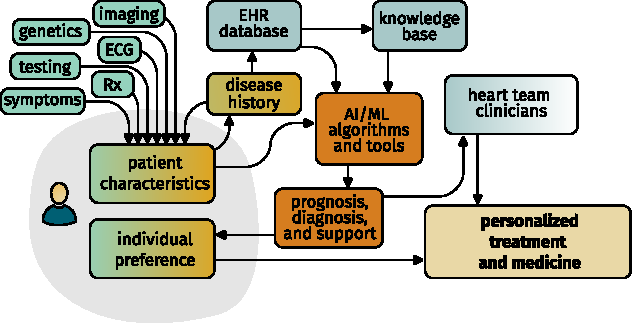
\includegraphics{graphics/precision-cardiology}
    \label{fig:precision-cardiology}
    \setfloatalignment{t}
    \vspace{-3em}
\end{figure}
% ←

The central elements of this precision cardiology workflow is:
\begin{enumerate*}
    \item big data collection and organization
    \item computer-based clinical tools and algorithms
    \item implementation of these tools in clinical decision making
\end{enumerate*}.
In the research underlying this thesis, 
the primary emphasis have been on (i) and (ii),
but without (iii) the advances of precision medicine
will remain mostly academic in scope.
The challenges and future perspectives of the clinical implementation
will be discussed later in the thesis.
Focusing on the first two elements, 
how do we derive tools and algorithms from big datasets?

